\documentclass{beamer}

\mode<presentation>
{
   \usetheme{EEng}
%   \usetheme{Warsaw}
  \setbeamercovered{transparent}
  \setbeamercolor{background canvas}{bg=black!0}
}

\usepackage{enumerate}
\usepackage{graphics}
\usepackage{ucs}
\usepackage[utf8x]{inputenc}
\usepackage[english]{babel}
\usepackage{amsmath}
\usepackage{amsfonts}
\usepackage{xcolor}
\usepackage{pgf}
\usepackage{hyperref}
\usepackage{url}
\usepackage{multicol}   % add-on
\usepackage{boxedminipage} 
\usepackage{indentfirst}   % add-on
\usepackage{float}
\usepackage[all]{xypic}
\usepackage{listings}
\usepackage{verbatim}
\usepackage{boxedminipage}

% % % inicio do listings e ref
\definecolor{darkblue}{rgb}{0,0,0.6}
\definecolor{gray_ulisses}{gray}{0.55}
\definecolor{castanho_ulisses}{rgb}{0.71,0.33,0.14}
\definecolor{preto_ulisses}{rgb}{0.41,0.20,0.04}
\definecolor{green_ulises}{rgb}{0.2,0.75,0}

\hypersetup{
	a4paper,
	pdftex,
	bookmarks,
	colorlinks,
    citecolor=darkblue,
    linkcolor=darkblue,
    urlcolor=darkblue,
    filecolor=darkblue
}

\lstdefinelanguage{Terminall} {
       basicstyle=\scriptsize\ttfamily,
       breaklines=true,
       breakautoindent=false,
       showstringspaces=false
}
\lstdefinelanguage{Terminal} {
       basicstyle=\tiny\ttfamily,
       breaklines=true,
       breakautoindent=false,
       showstringspaces=false
}
% % % fim do listings e ref

% % % inicio da definicao de comandos
\newcommand{\ixload}{\emph{IxLoad}}
\newcommand{\ixos}{\emph{IxOS}}
\newcommand{\ats}{\emph{ATS}}
\newcommand{\autoeasy}{\emph{AutoEASY}}
\newcommand{\ixia}{\emph{Ixia}}
\newcommand{\http}{\emph{HTTP}}
\newcommand{\ftp}{\emph{FTP}}
\newcommand{\ssl}{\emph{SSL}}
\newcommand{\pop}{\emph{POP$3$}}
\newcommand{\smtp}{\emph{SMTP}}
\newcommand{\fpm}{\emph{FPM}}
\newcommand{\sfpm}{\emph{SFPM}}
\newcommand{\ffpm}{\emph{FFPM}}
\newcommand{\cisco}{\emph{Cisco}}
% % % fim da definicao de comandos

\title{SAAP - Software para Análise e Avaliação de Programas}
\author{José Pedro Silva \and
Pedro Faria \and
Ulisses Costa
}

\date{\today}
\institute{Engenharia de Linguagens\\
Projecto integrado
}

\AtBeginSubsection[] {
  \begin{frame}<beamer>
    \frametitle{Index}
    \scriptsize{\tableofcontents[currentsection,currentsubsection]}
  \end{frame}
}

\AtBeginSection[] {
  \begin{frame}<beamer>
    \frametitle{Index}
    \scriptsize{\tableofcontents[currentsection]}
  \end{frame}
}
\begin{document}
\begin{frame}
   \titlepage
\end{frame}

\section{Motivação e Tecnologias}
\pgfdeclareimage[width=.8\textwidth]{topo}{images/topo}

\begin{frame} \frametitle{Motivação e Objectivos}
Aprofundar e demonstrar conhecimentos em:
\begin{itemize}
\item Desenhar arquitectura de um sistema de informação
\item Desenvolvimento web
\item Linguagens de Scripting
\item Bases de dados
\item Processamentos de texto
\end{itemize}
\end{frame}

\begin{frame} \frametitle{Tecnologia}
Principais ferramentas a usar:
\begin{itemize}
\item RoR - interface web
\item Perl - scripting
\item DB2 - motor de base de dados
\item Haskell
\end{itemize}
\end{frame}

\section{Contextualização}
\begin{frame} \frametitle{Descrição do Sistema}
Descrição do sistema e funcionalidades:
\begin{itemize}
\item Disponivel através de uma interface web
\item Criação de concursos e enunciados
\item Permite a submissão de programas
\item Avalia os programas submetidos
\item Gera métricas para programas existentes no sistema
\end{itemize}
\end{frame}

\begin{frame} \frametitle{Utilizadores do sistema - Docente}
\begin{itemize}
\item Pode criar, editar e eliminar concursos e enunciados
\item Pedir ao sistema para gerar métricas
\item Consultar todo o tipo de resultados
\end{itemize}
\end{frame}

\begin{frame} \frametitle{Utilizadores do sistema}
\begin{description}
\item[Admin] Entidade com mais poder no sistema, pode criar contas para docentes
\item[Grupo] Pode submeter ficheiros que serão avaliados pelo sistema
\end{description}
\end{frame}

\section{Modelação}
\begin{frame} \frametitle{Modelação informal da arquitectura}
\begin{figure}[htbp]
\begin{center}
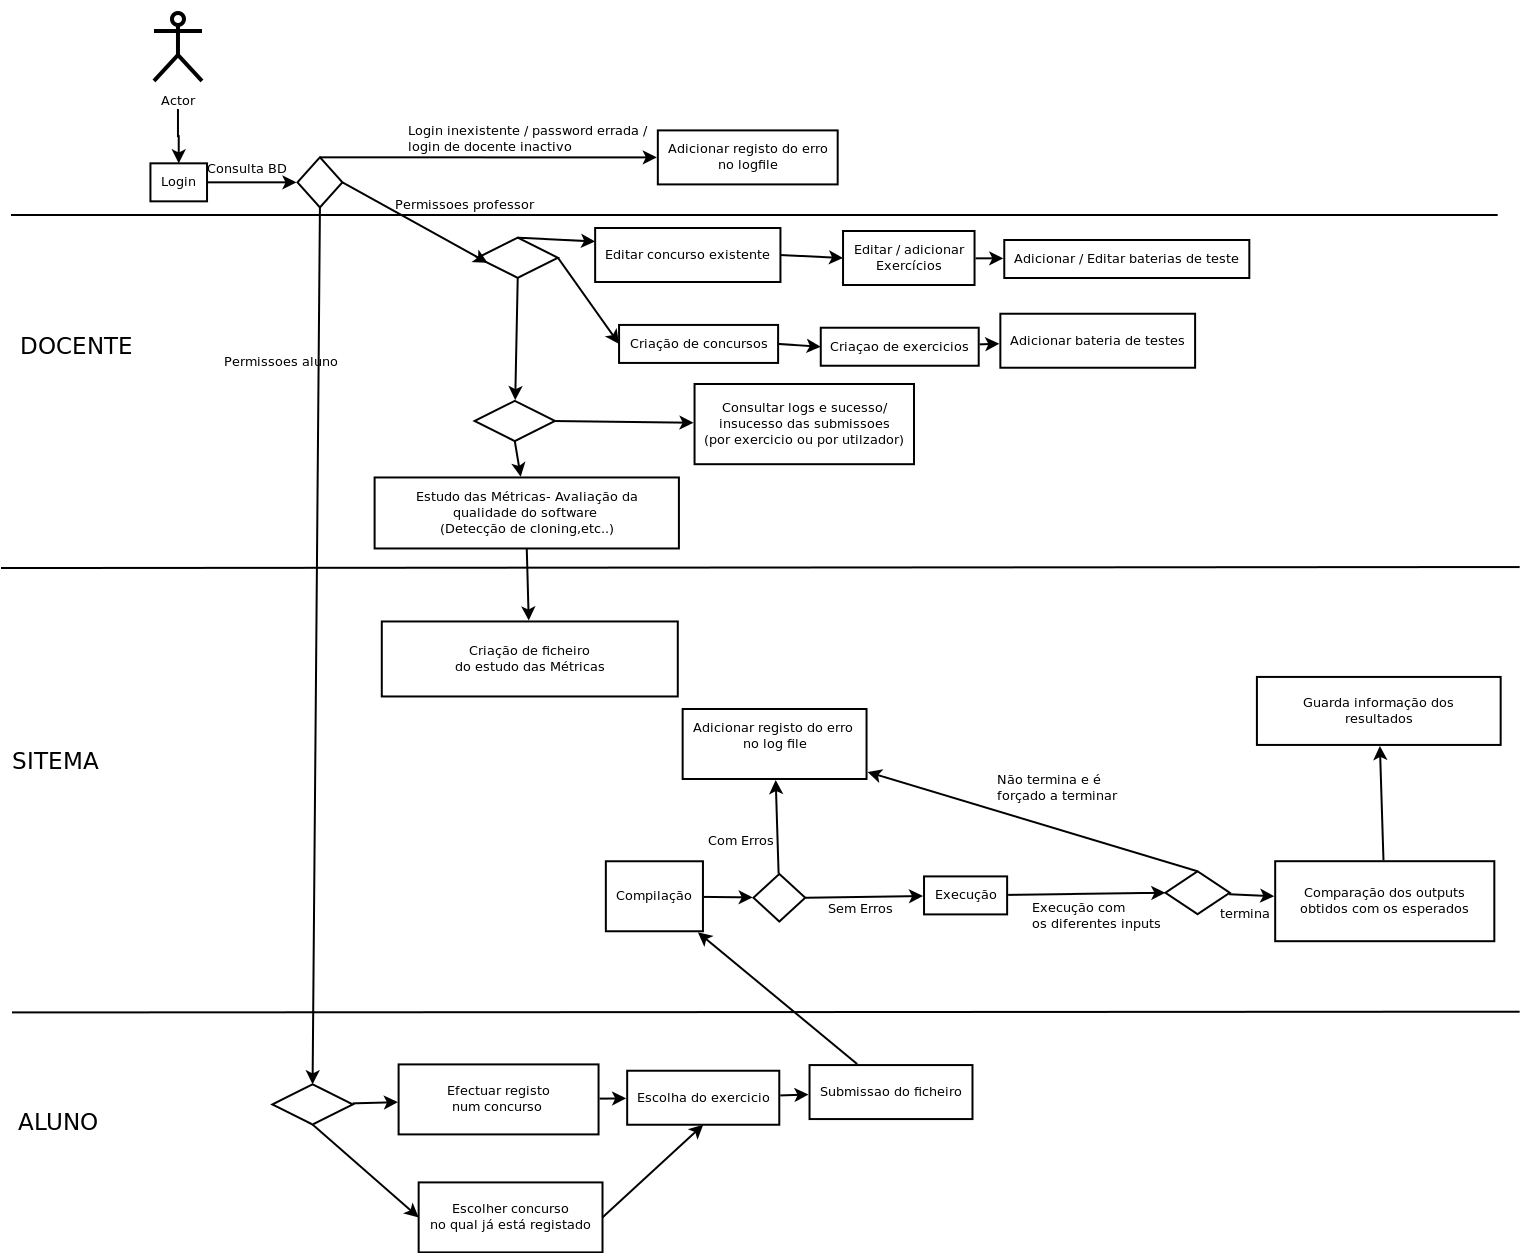
\includegraphics[width=0.8\textwidth]{../report1/Images/EL-PI}
\end{center}
\end{figure}
\end{frame}

\begin{frame} \frametitle{Modelação formal}
AFOGA-TE EM FORMALISMOS PRH
\end{frame}

\subsection{Modelação de dados}
\begin{frame} \frametitle{Modelo de dados - Grupo e Doecente/Admin}
\begin{figure}[htbp]
\begin{center}
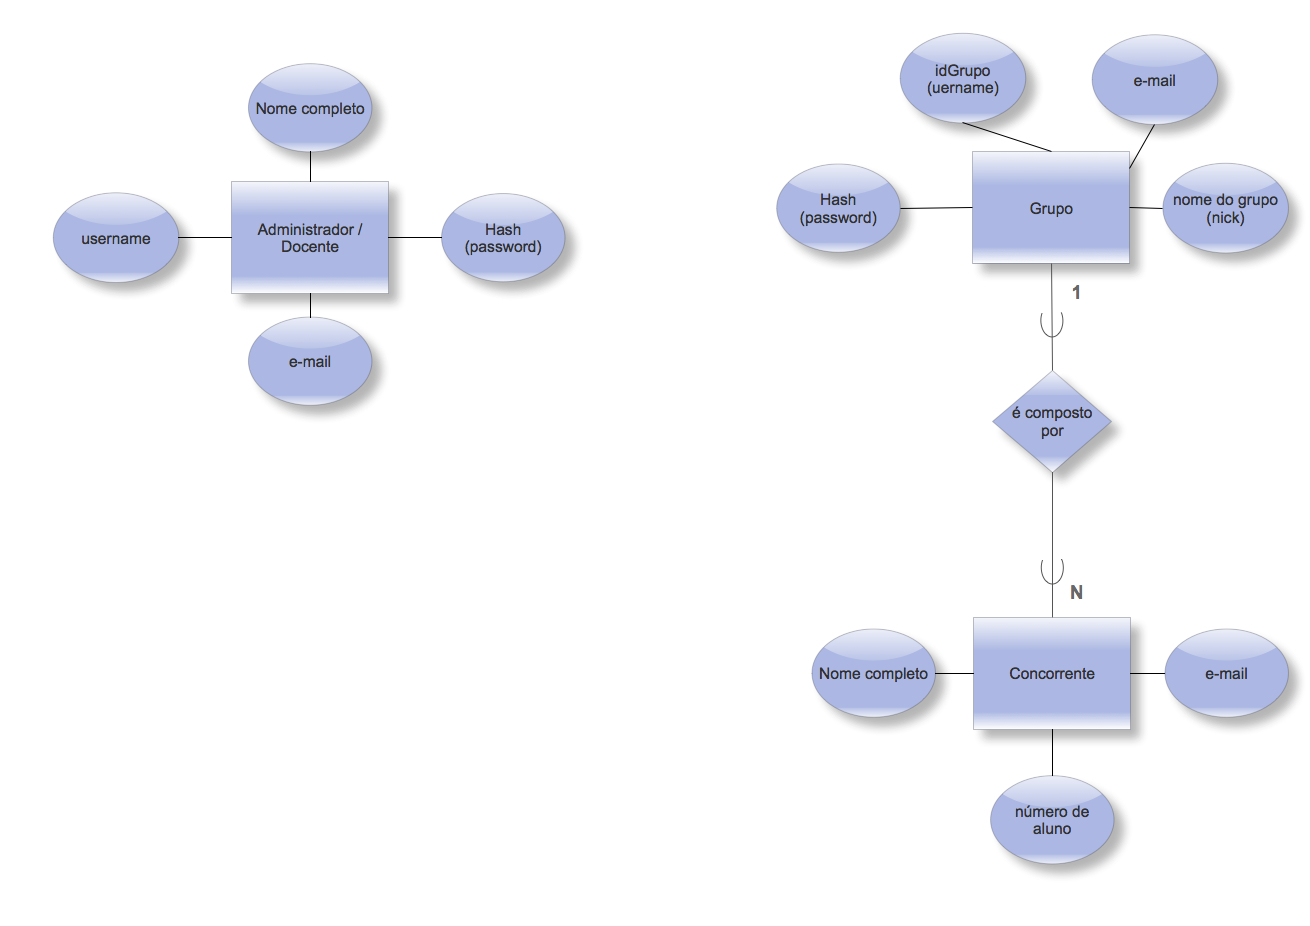
\includegraphics[width=0.9\textwidth]{../report1/Images/grupo-docente}
\end{center}
\end{figure}
\end{frame}

\begin{frame} \frametitle{Modelo de dados - Concurso, tentativa e enunciado}
\begin{figure}[htbp]
\begin{center}
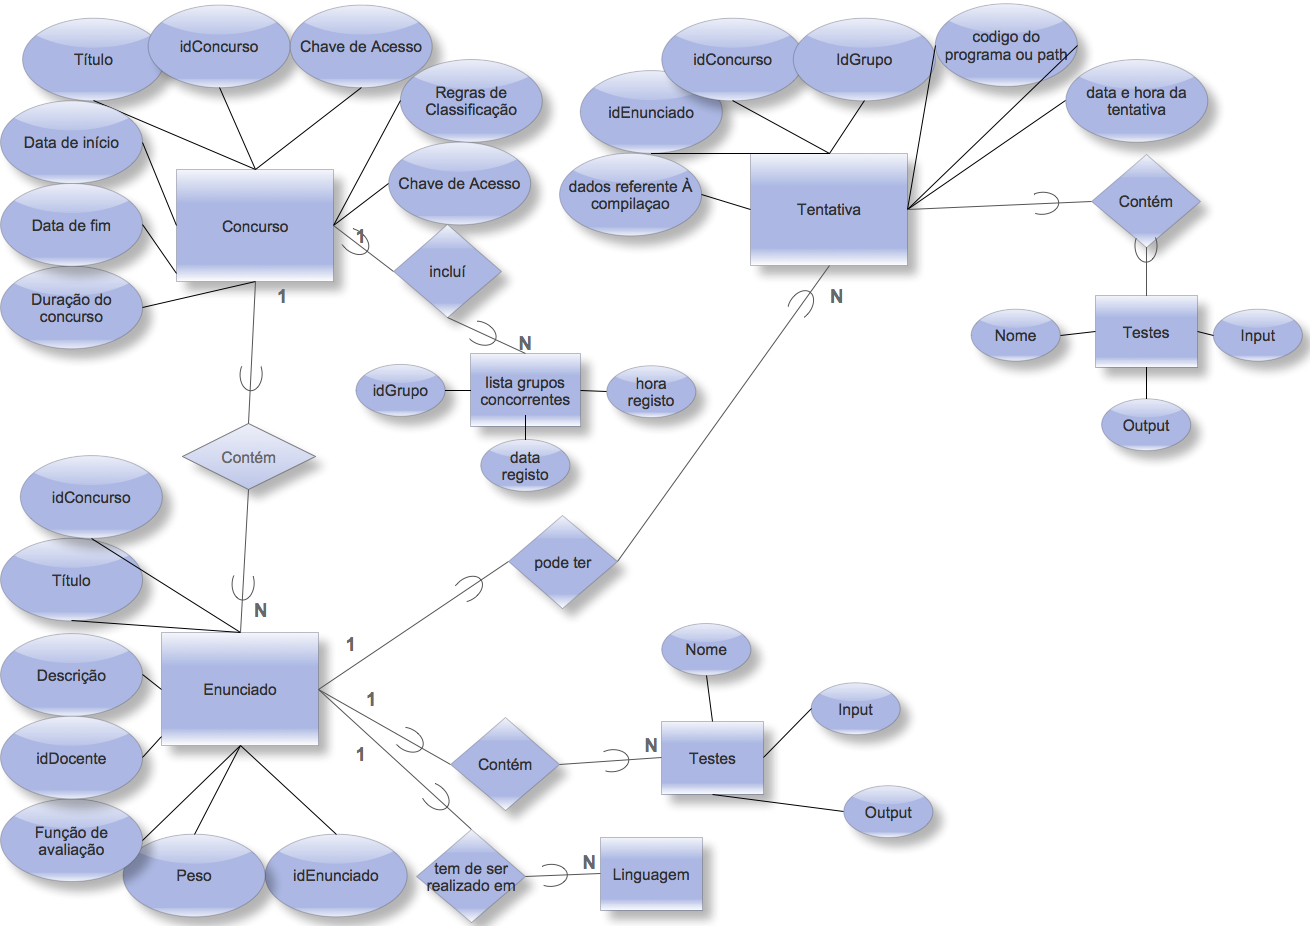
\includegraphics[width=0.9\textwidth]{../report1/Images/concurso-enunciado}
\end{center}
\end{figure}
\end{frame}

\begin{frame}[fragile] \frametitle{Modelo de dados - XML - Enunciado}
\begin{lstlisting}[language=XML,basicstyle=\tiny,breaklines=true]
<?xm l version="1.0" encoding="UTF-8"?>
<Enunciado xmlns:xsi="http://www.w3.org/2001/XMLSchema-instance"
    xsi:noNamespaceSchemaLocation="enunciado.xsd">
    <idConcurso> 1 </idConcurso>
    <Peso>20</Peso>
    <Titulo> Exercicio 1 </Titulo>
    <Descricao> Some os numeros que lhe sao passados como argumento, e apresente o resultado. </Descricao>
    <Exemplo>Input: 1 1 1 1 1   Output: 5</Exemplo>
    <Docente> PRH </Docente>
    <FuncAval>Diff</FuncAval>  
    <Linguagens> 
        <Linguagem>C</Linguagem>        
    </Linguagens> 
\end{lstlisting}
\end{frame}

\begin{frame}[fragile] \frametitle{Modelo de dados - XML - Enunciado - Part2}
\begin{lstlisting}[language=XML,basicstyle=\tiny,breaklines=true]
    <Dict>
        <Teste>
            <Nome>Lista vazia</Nome>
            <Input></Input>
            <Output>0</Output>
        </Teste>
        <Teste>
            <Nome>Lista c/ 1 elem</Nome>
            <Input>1</Input>
            <Output>1</Output>
        </Teste>
        <Teste>
            <Nome>Lista c/ varios elem</Nome>
            <Input> 2 3 4 5 </Input>
            <Output>14</Output>
        </Teste>
    </Dict>
</Enunciado>
\end{lstlisting}
\end{frame}

\begin{frame}[fragile] \frametitle{Modelo de dados - XML - Tentativa}
\begin{lstlisting}[language=XML,basicstyle=\tiny,breaklines=true]
<?xm l version="1.0" encoding="UTF-8"?>
<Enunciado xmlns:xsi="http://www.w3.org/2001/XMLSchema-instance"
    xsi:noNamespaceSchemaLocation="tentativa.xsd">
    <idConcurso>1</idConcurso>
    <idEnunciado>1</idEnunciado>
    <idGrupo>36</idGrupo>
    
    <data>2010-12-08</data>
    <hora>16:33:00</hora>
    
    <compilou>1</compilou>
\end{lstlisting}
\end{frame}

\begin{frame}[fragile] \frametitle{Modelo de dados - XML - Tentativa - Part2}
\begin{lstlisting}[language=XML,basicstyle=\tiny,breaklines=true]
    <Dict>
        <Teste>
            <Nome>Lista vazia</Nome>
            <Input></Input>
            <Output>0</Output>
        </Teste>
        <Teste>
            <Nome>Lista c/ 1 elem</Nome>
            <Input>1</Input>
            <Output>1</Output>
        </Teste>
        <Teste>
            <Nome>Lista c/ varios elem</Nome>
            <Input> 2 3 4 5 </Input>
            <Output>14</Output>
        </Teste>
    </Dict>
    <pathMetricas>sasas</pathMetricas>
\end{lstlisting}
\end{frame}

\begin{frame}[fragile] \frametitle{Modelo de dados - XML - Tentativa - Part3}
\begin{lstlisting}[language=XML,basicstyle=\tiny,breaklines=true]
    <codigoFonte>
        <nome>prog.c</nome>
        <codigo>
            <![CDATA[
            #include <stdio.h>
            
            ...restante codigo...
            
            ]]>
        </codigo>
    </codigoFonte>
        
</Enunciado>
\end{lstlisting}
\end{frame}

\begin{frame}[fragile] \frametitle{Modelo de dados - XSD - Enunciado}
\begin{lstlisting}[language=XML,basicstyle=\tiny,breaklines=true]
<ed:element name="Peso" default="25">
  <ed:simpleType>
    <ed:restriction base="ed:integer">
      <ed:minInclusive value="0"/>
      <ed:maxInclusive value="100"/>
    </ed:restriction>
  </ed:simpleType>
</ed:element>
\end{lstlisting}
\end{frame}

\begin{frame}[fragile] \frametitle{Modelo de dados - XSD - Linguagem}
\begin{lstlisting}[language=XML,basicstyle=\tiny,breaklines=true]
<ed:element name="Linguagem" maxOccurs="unbounded">
    <ed:simpleType>
    <ed:restriction base="ed:string">
        <ed:enumeration value="C"/>
        <ed:enumeration value="Java"/>
        <ed:enumeration value="Haskell"/>
    </ed:restriction>
    </ed:simpleType>
</ed:element>
\end{lstlisting}
\end{frame}

\begin{frame}[fragile] \frametitle{Modelo de dados - XSD - Tentativa}
\begin{lstlisting}[language=XML,basicstyle=\tiny,breaklines=true]
<tt:element name="Dict">
    <tt:complexType>
    <tt:sequence>
        <tt:element name="Teste" maxOccurs="unbounded">
        <tt:complexType>
            <tt:sequence>
            <tt:element name="Nome" type="tt:string"/>
            <tt:element name="Input" type="tt:string"/>
            <tt:element name="Output" type="tt:string"/>
            </tt:sequence>
        </tt:complexType>
        </tt:element>
    </tt:sequence>
    </tt:complexType>
</tt:element>
\end{lstlisting}
\end{frame}

\section*{Perguntas}
\begin{frame} \frametitle{Perguntas}
\begin{center}\huge{?}\end{center}
\end{frame}

\end{document}
